% ###################################################################################################
% Chapter 7 - Combat and Conflict Resolution
% ###################################################################################################
\chapter{Conflict Mechanics}

% Chapter-wide image
\begin{center}
    
\includegraphics[width=\textwidth]{./images/combat01.pdf}
\end{center}

In \textit{Eidos}, the combat is based on the ideas presented in this \href{https://www.youtube.com/watch?v=0o5vWmoS3KU&ab_channel=SimplyWyvern}{video}. Basically, the combat needs to be a part of the narrative, not a mini-game that creates transitions in the game. So there is nothing of initiative rolls nor anything like that. In the world of \textit{Eidos}, combat is a dynamic and immersive experience that forms an integral part of the gameplay. The combat system in \textit{Eidos} is meticulously crafted to simulate realistic combat scenarios, with mechanics that emphasize tactical decision-making and narrative engagement.

\section{Turn Structure}

Combat in Eidos follows a fluid turn structure, allowing for seamless interaction between players and the game master. Unlike traditional turn-based systems, Eidos prioritizes moment-to-moment decision-making, where players and the GM exchange actions and reactions in real-time. This approach enhances the narrative flow of combat scenes, fostering a sense of urgency and immersion.

\section{Conflict Resolution}

Conflict in Eidos is resolved through a combination of dice rolls and narrative storytelling. The core engine is based on a \textbf{2d20 roll}. When a character attempts a challenging task, the player rolls two 20-sided dice, adds the two results together, and adds the relevant Attribute Modifier and Skill Modifier.

\begin{center}
    \textbf{Core Formula: } $2\text{d}20 + \text{Attribute Modifier} + \text{Skill Modifier}$
\end{center}

This total is compared against a Target Number (TN) set by the Game Master (GM) based on the narrative difficulty:

\begin{itemize}
    \item \textbf{Very easy:} Target number 05
    \item \textbf{Easy:} Target number 10
    \item \textbf{Moderate:} Target number 15
    \item \textbf{Difficult:} Target number 20
    \item \textbf{Hard:} Target number 25
    \item \textbf{Very hard:} Target number 30
    \item \textbf{Extremely hard:} Target number 35
    \item \textbf{Nearly impossible:} Target number 39
\end{itemize}

\subsection{Character Attributes}

All characters are defined by four core attributes, representing their natural physical and mental capabilities. During character creation, players distribute the Standard Array of modifiers: \textbf{+2, +1, 0, -1} among these attributes:

\begin{description}
    \item[Strength (STR):] Physical brawn, lifting power, muscle endurance, and blunt/impact damage.
    \item[Agility (AGI):] Reflexes, speed, bodily coordination, stealth, and light/fenced weaponry precision.
    \item[Mind (MND):] Intellect, memory, academic knowledge, sensory perception, and spellcasting ability.
    \item[Presence (PRE):] Charisma, social influence, leadership capacity, and mental willpower.
\end{description}

\subsection{Combat Rolls and Defenses}

In Eidos, combat is seamless and narrative-focused. There are no static turn orders or initiative rolls; action flows logically based on player decisions and narrative prompts. 

When a character attacks an opponent, the player rolls an attack check:
\begin{center}
    \textbf{Attack Roll:} $2\text{d}20 + \text{AGI or STR} + \text{Combat Skill}$
\end{center}
* \textbf{Agility} is used for light, fencing, or ranged weapons (e.g., daggers, shortswords, bows).
* \textbf{Strength} is used for heavy impact or two-handed weapons (e.g., axes, maces, greatswords).

An attack succeeds if it meets or exceeds the defender's \textbf{Defense}. A defender can choose to use either passive or active defenses:

\begin{itemize}
    \item \textbf{Passive Defense (Static):} The defender relies on their passive posture and positioning. 
    \begin{center}
        \textbf{Static Defense:} $10 + \text{AGI} + \text{Shield Modifier}$
    \end{center}
    \item \textbf{Active Defense (Roll):} The defender spends their reaction to actively parry, dodge, or block the strike. They roll:
    \begin{center}
        \textbf{Active Defense Check:} $2\text{d}20 + \text{AGI (or STR for shielding)} + \text{Athletics/Combat Skill}$
    \end{center}
    If the Active Defense roll meets or exceeds the attacker's roll, the attack is fully avoided or blocked.
\end{itemize}

\subsection{Critical Hits and Injuries}

If an attack roll is successful and hits, the attacker rolls a 1d20 on the corresponding region and damage injury table (e.g., "Cutting in the Head"). 

A \textbf{Critical Hit} occurs when:
\begin{enumerate}
    \item A player rolls a natural 20 on either of the two d20s during their attack check, OR
    \item The final attack roll exceeds the defender's Defense by 10 or more.
\end{enumerate}

When a Critical Hit is scored, the defender is exposed to massive damage. Eidos' critical injury tables define severe outcomes ranging from minor scalp wounds to decapitation and instant death. Armor reduces the severity of these rolls directly (see Chapter 6).

\subsection{Types of Injury}

Types of injury include several categories based on the nature of the harm inflicted. \textbf{Cutting} involves damage from sharp-edged weapons, such as swords or knives, which can cause deep lacerations. \textbf{Stabbing} refers to injuries from piercing weapons, like spears or daggers, that penetrate deeply into the body. \textbf{Impact} injuries result from blunt force or crushing attacks, often leading to bruising or broken bones. \textbf{Fire} damage is caused by burns or heat sources, leaving severe burns and potentially long-term tissue damage. \textbf{Acid} injuries come from exposure to corrosive acids or chemicals, which can eat away at skin and muscle. \textbf{Poison} represents harm caused by toxic substances that can weaken or kill through systemic effects. Finally, \textbf{Fall} injuries occur when someone falls from a significant height, often causing fractures, sprains, or other trauma.

\subsection{Injury Places}

\begin{itemize}
    \item \textbf{Head:} The uppermost part of the body.
    \item \textbf{Torso:} The main part of the body, including the chest.
    \item \textbf{Left Arm:} The left arm and hand.
    \item \textbf{Right Arm:} The right arm and hand.
    \item \textbf{Left Leg:} The left leg and foot.
    \item \textbf{Right Leg:} The right leg and foot.
    \item \textbf{Abdomen:} The area between the chest and pelvis.
    \item \textbf{Back:} The rear part of the torso.
    \item \textbf{Neck:} The part connecting the head to the body.
    \item \textbf{Face:} The front of the head, including facial features.
\end{itemize}

\begin{figure}[h]
    \centering
    
\includegraphics[width=\textwidth]{./images/combat03.pdf}
    % \caption{Inline Example Image}
\end{figure}

\subsection{Cutting in the Head}

\begin{description}[labelwidth=1.5em, leftmargin=*, itemsep=0.3em]
    \item[01 -] Minor scalp laceration, blood trickling. \textit{Recovery Time:} 1d4 hours. \textit{Scars:} Light scar.
    \item[02 -] Shallow cut on forehead, slight bleeding. \textit{Recovery Time:} 1d4 hours. \textit{Scars:} Small scar.
    \item[03 -] Ear nicked, minor pain and bleeding. \textit{Recovery Time:} 1d4 hours. \textit{Scars:} Tiny scar.
    \item[04 -] Cheek grazed, minor discomfort. \textit{Recovery Time:} 1d4 hours. \textit{Scars:} Faint scar.
    \item[05 -] Eyebrow cut, minor blood and irritation. \textit{Recovery Time:} 1d4 hours. \textit{Scars:} Light scar.
    \item[06 -] Nose scratched, slight bleeding. \textit{Recovery Time:} 1d4 hours. \textit{Scars:} Small scar.
    \item[07 -] Chin cut, stinging pain and minor blood. \textit{Recovery Time:} 1d4 hours. \textit{Scars:} Tiny scar.
    \item[08 -] Forehead gash, bleeding and moderate pain. \textit{Recovery Time:} 1d4 hours. \textit{Scars:} Faint scar.
    \item[09 -] Scalp tear, bleeding and headache. \textit{Recovery Time:} 1d4 hours. \textit{Scars:} Light scar.
    \item[10 -] Lip cut, bleeding and mild pain. \textit{Recovery Time:} 1d4 hours. \textit{Scars:} Small scar.
    \item[11 -] Deep facial wound, potential scarring. \textit{Recovery Time:} 1d4 days. \textit{Scars:} Visible scar.
    \item[12 -] Eye injured, risk of blindness. \textit{Recovery Time:} 1d4 days. \textit{Scars:} Disfiguring scar.
    \item[13 -] Skull fracture, severe headache. \textit{Recovery Time:} 1d4 weeks. \textit{Scars:} Permanent damage.
    \item[14 -] Head gash, risk of infection. \textit{Recovery Time:} 1d4 weeks. \textit{Scars:} Deep scar.
    \item[15 -] Severed artery, immediate death. \textit{Recovery Time:} Instant death. \textit{Scars:} N/A.
    \item[16 -] Severe brain injury, instant unconsciousness. \textit{Recovery Time:} Instant death. \textit{Scars:} N/A.
    \item[17 -] Instant brain death, no chance of revival. \textit{Recovery Time:} Instant death. \textit{Scars:} N/A.
    \item[18 -] Severe cranial trauma, instant death. \textit{Recovery Time:} Instant death. \textit{Scars:} N/A.
    \item[19 -] Critical hit, catastrophic brain damage. \textit{Recovery Time:} Instant death. \textit{Scars:} N/A.
    \item[20 -] Critical hit, brain pierced, instant death. \textit{Recovery Time:} Instant death. \textit{Scars:} N/A.
\end{description}

\begin{figure}[h]
    \centering
    
\includegraphics[width=\textwidth]{./images/combat06.pdf}
    % \caption{Inline Example Image}
\end{figure}

\subsection{Cutting in the Torso}

\begin{description}[labelwidth=1.5em, leftmargin=*, itemsep=0.4em]
    \item[01 -] Superficial chest graze, minor pain. \textit{Recovery Time:} 1d4 hours. \textit{Scars:} Faint scar.
    \item[02 -] Light abdominal scratch, discomfort. \textit{Recovery Time:} 1d4 hours. \textit{Scars:} Small scar.
    \item[03 -] Minor rib cut, mild pain and shallow bleeding. \textit{Recovery Time:} 1d4 hours. \textit{Scars:} Tiny scar.
    \item[04 -] Skin nicked on side, slight irritation. \textit{Recovery Time:} 1d4 hours. \textit{Scars:} Faint scar.
    \item[05 -] Chest cut, moderate pain and minor bleeding. \textit{Recovery Time:} 1d4 hours. \textit{Scars:} Light scar.
    \item[06 -] Abdominal laceration, blood trickling. \textit{Recovery Time:} 1d4 hours. \textit{Scars:} Small scar.
    \item[07 -] Side wound, moderate pain and bleeding. \textit{Recovery Time:} 1d4 hours. \textit{Scars:} Tiny scar.
    \item[08 -] Deep chest gash, significant bleeding. \textit{Recovery Time:} 1d4 days. \textit{Scars:} Faint scar.
    \item[09 -] Rib gash, severe pain and bleeding. \textit{Recovery Time:} 1d4 days. \textit{Scars:} Light scar.
    \item[10 -] Abdominal cut, potential scarring. \textit{Recovery Time:} 1d4 days. \textit{Scars:} Small scar.
    \item[11 -] Organ grazed, risk of infection. \textit{Recovery Time:} 1d4 weeks. \textit{Scars:} Deep scar.
    \item[12 -] Punctured lung, difficulty breathing. \textit{Recovery Time:} 1d4 weeks. \textit{Scars:} Permanent damage.
    \item[13 -] Severe internal injury, risk of shock. \textit{Recovery Time:} 1d4 weeks. \textit{Scars:} Visible scar.
    \item[14 -] Aorta nicked, rapid blood loss. \textit{Recovery Time:} Instant death. \textit{Scars:} N/A.
    \item[15 -] Heart pierced, immediate death. \textit{Recovery Time:} Instant death. \textit{Scars:} N/A.
    \item[16 -] Severed spinal cord, instant paralysis. \textit{Recovery Time:} Instant death. \textit{Scars:} N/A.
    \item[17 -] Major organ rupture, instant internal bleeding. \textit{Recovery Time:} Instant death. \textit{Scars:} N/A.
    \item[18 -] Critical hit, catastrophic internal damage. \textit{Recovery Time:} Instant death. \textit{Scars:} N/A.
    \item[19 -] Critical hit, vital organs obliterated. \textit{Recovery Time:} Instant death. \textit{Scars:} N/A.
    \item[20 -] Critical hit, torso sliced open, instant death. \textit{Recovery Time:} Instant death. \textit{Scars:} N/A.
\end{description}

\subsection{Cutting in the Arms}

\begin{description}[labelwidth=1.5em, leftmargin=*, itemsep=0.4em]
    \item[01 -] Superficial arm graze, minor discomfort. \textit{Recovery Time:} 1d4 hours. \textit{Scars:} Faint scar.
    \item[02 -] Light forearm scratch, slight pain. \textit{Recovery Time:} 1d4 hours. \textit{Scars:} Small scar.
    \item[03 -] Minor hand cut, mild bleeding. \textit{Recovery Time:} 1d4 hours. \textit{Scars:} Tiny scar.
    \item[04 -] Skin nicked on upper arm, slight irritation. \textit{Recovery Time:} 1d4 hours. \textit{Scars:} Faint scar.
    \item[05 -] Elbow grazed, moderate pain and minor bleeding. \textit{Recovery Time:} 1d4 hours. \textit{Scars:} Light scar.
    \item[06 -] Wrist scratched, slight bleeding. \textit{Recovery Time:} 1d4 hours. \textit{Scars:} Small scar.
    \item[07 -] Finger cut, stinging pain and minor bleeding. \textit{Recovery Time:} 1d4 hours. \textit{Scars:} Tiny scar.
    \item[08 -] Deep forearm gash, significant bleeding. \textit{Recovery Time:} 1d4 days. \textit{Scars:} Faint scar.
    \item[09 -] Upper arm cut, severe pain and bleeding. \textit{Recovery Time:} 1d4 days. \textit{Scars:} Light scar.
    \item[10 -] Hand laceration, potential scarring. \textit{Recovery Time:} 1d4 days. \textit{Scars:} Small scar.
    \item[11 -] Tendon nicked, risk of permanent damage. \textit{Recovery Time:} 1d4 weeks. \textit{Scars:} Deep scar.
    \item[12 -] Arterial wound, rapid blood loss. \textit{Recovery Time:} Instant death. \textit{Scars:} N/A.
    \item[13 -] Hand mutilation, high risk of infection. \textit{Recovery Time:} Instant death. \textit{Scars:} N/A.
    \item[14 -] Severe muscle damage, limited use of arm. \textit{Recovery Time:} 1d4 weeks. \textit{Scars:} Permanent damage.
    \item[15 -] Hand severed, instant death. \textit{Recovery Time:} Instant death. \textit{Scars:} N/A.
    \item[16 -] Critical hit, arm sliced off, instant death. \textit{Recovery Time:} Instant death. \textit{Scars:} N/A.
    \item[17 -] Critical hit, arm mutilated, instant death. \textit{Recovery Time:} Instant death. \textit{Scars:} N/A.
    \item[18 -] Critical hit, arteries severed, instant death. \textit{Recovery Time:} Instant death. \textit{Scars:} N/A.
    \item[19 -] Critical hit, shattered bones, instant death. \textit{Recovery Time:} Instant death. \textit{Scars:} N/A.
    \item[20 -] Critical hit, arm disintegrated, instant death. \textit{Recovery Time:} Instant death. \textit{Scars:} N/A.
\end{description}

\begin{figure}[h]
    \centering
    \includegraphics[width=\textwidth]{./images/combat07.pdf}
    % \caption{Inline Example Image}
\end{figure}

\subsection{Cutting in the Legs}

\begin{description}[labelwidth=1.5em, leftmargin=*, itemsep=0.4em]
    \item[1 -] Superficial thigh graze, minor discomfort. \textit{Recovery Time:} 1d4 hours. \textit{Scars:} Faint scar.
    \item[2 -] Light calf scratch, slight pain. \textit{Recovery Time:} 1d4 hours. \textit{Scars:} Small scar.
    \item[3 -] Minor ankle cut, mild bleeding. \textit{Recovery Time:} 1d4 hours. \textit{Scars:} Tiny scar.
    \item[4 -] Skin nicked on shin, slight irritation. \textit{Recovery Time:} 1d4 hours. \textit{Scars:} Faint scar.
    \item[5 -] Knee grazed, moderate pain and minor bleeding. \textit{Recovery Time:} 1d4 hours. \textit{Scars:} Light scar.
    \item[6 -] Heel scratched, slight bleeding. \textit{Recovery Time:} 1d4 hours. \textit{Scars:} Small scar.
    \item[7 -] Toe cut, stinging pain and minor bleeding. \textit{Recovery Time:} 1d4 hours. \textit{Scars:} Tiny scar.
    \item[8 -] Deep thigh gash, significant bleeding. \textit{Recovery Time:} 1d4 days. \textit{Scars:} Faint scar.
    \item[9 -] Calf cut, severe pain and bleeding. \textit{Recovery Time:} 1d4 days. \textit{Scars:} Light scar.
    \item[10 -] Ankle laceration, potential scarring. \textit{Recovery Time:} 1d4 days. \textit{Scars:} Small scar.
    \item[11 -] Tendon severed, risk of permanent damage. \textit{Recovery Time:} 1d4 weeks. \textit{Scars:} Deep scar.
    \item[12 -] Arterial wound, rapid blood loss. \textit{Recovery Time:} Instant death. \textit{Scars:} N/A.
    \item[13 -] Leg mutilation, high risk of infection. \textit{Recovery Time:} Instant death. \textit{Scars:} N/A.
    \item[14 -] Severe muscle damage, limited mobility. \textit{Recovery Time:} 1d4 weeks. \textit{Scars:} Permanent damage.
    \item[15 -] Leg severed, instant death. \textit{Recovery Time:} Instant death. \textit{Scars:} N/A.
    \item[16 -] Critical hit, leg sliced off, instant death. \textit{Recovery Time:} Instant death. \textit{Scars:} N/A.
    \item[17 -] Critical hit, leg mutilated, instant death. \textit{Recovery Time:} Instant death. \textit{Scars:} N/A.
    \item[18 -] Critical hit, arteries severed, instant death. \textit{Recovery Time:} Instant death. \textit{Scars:} N/A.
    \item[19 -] Critical hit, shattered bones, instant death. \textit{Recovery Time:} Instant death. \textit{Scars:} N/A.
    \item[20 -] Critical hit, leg disintegrated, instant death. \textit{Recovery Time:} Instant death. \textit{Scars:} N/A.
\end{description}

\begin{figure}[h]
    \centering
    
\includegraphics[width=\textwidth]{./images/combat04.pdf}
    % \caption{Inline Example Image}
\end{figure}

\subsection{Cutting in the Abdomen}

\begin{description}[labelwidth=1.5em, leftmargin=*, itemsep=0.4em]
    \item[1 -] Superficial scratch, minor discomfort. \textit{Recovery Time:} 1d4 hours. \textit{Scars:} Light scar.
    \item[2 -] Shallow cut, light bleeding and mild pain. \textit{Recovery Time:} 1d4 hours. \textit{Scars:} Small scar.
    \item[3 -] Glancing blow, minimal bleeding. \textit{Recovery Time:} 1d4 hours. \textit{Scars:} Tiny scar.
    \item[4 -] Skin nicked, slight pain and minor bleeding. \textit{Recovery Time:} 1d4 hours. \textit{Scars:} Faint scar.
    \item[5 -] Grazed wound, bleeding and moderate pain. \textit{Recovery Time:} 1d4 hours. \textit{Scars:} Light scar.
    \item[6 -] Sliced flesh, steady bleeding and discomfort. \textit{Recovery Time:} 1d4 hours. \textit{Scars:} Small scar.
    \item[7 -] Deep cut, significant pain and bleeding. \textit{Recovery Time:} 1d4 hours. \textit{Scars:} Tiny scar.
    \item[8 -] Muscle incision, bleeding and throbbing pain. \textit{Recovery Time:} 1d4 hours. \textit{Scars:} Faint scar.
    \item[9 -] Torn flesh, profuse bleeding and severe pain. \textit{Recovery Time:} 1d4 days. \textit{Scars:} Light scar.
    \item[10 -] Severe laceration, risk of infection and agony. \textit{Recovery Time:} 1d4 days. \textit{Scars:} Small scar.
    \item[11 -] Ruptured muscle, intense pain and internal bleeding. \textit{Recovery Time:} 1d4 days. \textit{Scars:} Visible scar.
    \item[12 -] Organ grazed, danger of internal complications. \textit{Recovery Time:} 1d4 weeks. \textit{Scars:} Deep scar.
    \item[13 -] Severed artery, rapid blood loss and shock. \textit{Recovery Time:} 1d4 weeks. \textit{Scars:} Permanent damage.
    \item[14 -] Major organ damage, critical condition. \textit{Recovery Time:} 1d4 weeks. \textit{Scars:} Life-altering scar.
    \item[15 -] Perforated intestine, septicemia and extreme pain. \textit{Recovery Time:} Instant death. \textit{Scars:} N/A.
    \item[16 -] Ruptured kidney, internal hemorrhage and shock. \textit{Recovery Time:} Instant death. \textit{Scars:} N/A.
    \item[17 -] Impaled aorta, rapid exsanguination and agony. \textit{Recovery Time:} Instant death. \textit{Scars:} N/A.
    \item[18 -] Critical hit, disembowelment and instant death. \textit{Recovery Time:} Instant death. \textit{Scars:} N/A.
    \item[19 -] Critical hit, evisceration and instant death. \textit{Recovery Time:} Instant death. \textit{Scars:} N/A.
    \item[20 -] Critical hit, shredded organs and instant death. \textit{Recovery Time:} Instant death. \textit{Scars:} N/A.
\end{description}

\subsection{Cutting in the Back}

\begin{description}[labelwidth=1.5em, leftmargin=*, itemsep=0.4em]
    \item[1 -] Superficial scratch, minor discomfort. \textit{Recovery Time:} 1d4 hours. \textit{Scars:} Light scar.
    \item[2 -] Shallow cut, light bleeding and mild pain. \textit{Recovery Time:} 1d4 hours. \textit{Scars:} Small scar.
    \item[3 -] Skin grazed, slight pain and minor bleeding. \textit{Recovery Time:} 1d4 hours. \textit{Scars:} Tiny scar.
    \item[4 -] Flesh nicked, minor discomfort. \textit{Recovery Time:} 1d4 hours. \textit{Scars:} Faint scar.
    \item[5 -] Surface cut, bleeding and moderate pain. \textit{Recovery Time:} 1d4 hours. \textit{Scars:} Light scar.
    \item[6 -] Muscle graze, slight bleeding and irritation. \textit{Recovery Time:} 1d4 hours. \textit{Scars:} Small scar.
    \item[7 -] Deep cut, significant pain and bleeding. \textit{Recovery Time:} 1d4 hours. \textit{Scars:} Tiny scar.
    \item[8 -] Tendon nicked, bleeding and throbbing pain. \textit{Recovery Time:} 1d4 hours. \textit{Scars:} Faint scar.
    \item[9 -] Muscle laceration, bleeding and discomfort. \textit{Recovery Time:} 1d4 days. \textit{Scars:} Light scar.
    \item[10 -] Nerve cut, risk of partial paralysis and agony. \textit{Recovery Time:} 1d4 days. \textit{Scars:} Small scar.
    \item[11 -] Ruptured muscle, intense pain and internal bleeding. \textit{Recovery Time:} 1d4 days. \textit{Scars:} Visible scar.
    \item[12 -] Organ grazed, potential internal complications. \textit{Recovery Time:} 1d4 weeks. \textit{Scars:} Deep scar.
    \item[13 -] Major artery cut, rapid blood loss and shock. \textit{Recovery Time:} 1d4 weeks. \textit{Scars:} Permanent damage.
    \item[14 -] Spinal injury, paralysis risk and extreme pain. \textit{Recovery Time:} 1d4 weeks. \textit{Scars:} Life-altering scar.
    \item[15 -] Severed spine, instant paralysis and agony. \textit{Recovery Time:} Instant death. \textit{Scars:} N/A.
    \item[16 -] Critical hit, spine shattered, instant death. \textit{Recovery Time:} Instant death. \textit{Scars:} N/A.
    \item[17 -] Critical hit, spine pierced, instant death. \textit{Recovery Time:} Instant death. \textit{Scars:} N/A.
    \item[18 -] Critical hit, vital organ pierced, instant death. \textit{Recovery Time:} Instant death. \textit{Scars:} N/A.
    \item[19 -] Critical hit, disembowelment and instant death. \textit{Recovery Time:} Instant death. \textit{Scars:} N/A.
    \item[20 -] Critical hit, catastrophic spinal trauma and death. \textit{Recovery Time:} Instant death. \textit{Scars:} N/A.
\end{description}

\begin{figure}[h]
    \centering
    \includegraphics[width=\textwidth]{./images/combat08.pdf}
    % \caption{Inline Example Image}
\end{figure}

\subsection{Cutting in the Neck}

\begin{description}[labelwidth=1.5em, leftmargin=*, itemsep=0.4em]
    \item[1 -] Skin nick, minor discomfort. \textit{Recovery Time:} 1d4 hours. \textit{Scars:} Light scar.
    \item[2 -] Shallow cut, light bleeding and mild pain. \textit{Recovery Time:} 1d4 hours. \textit{Scars:} Small scar.
    \item[3 -] Neck graze, slight pain and minor bleeding. \textit{Recovery Time:} 1d4 hours. \textit{Scars:} Tiny scar.
    \item[4 -] Flesh cut, minor discomfort. \textit{Recovery Time:} 1d4 hours. \textit{Scars:} Faint scar.
    \item[5 -] Surface wound, bleeding and moderate pain. \textit{Recovery Time:} 1d4 hours. \textit{Scars:} Light scar.
    \item[6 -] Muscle nick, slight bleeding and irritation. \textit{Recovery Time:} 1d4 hours. \textit{Scars:} Small scar.
    \item[7 -] Deep gash, significant pain and bleeding. \textit{Recovery Time:} 1d4 hours. \textit{Scars:} Tiny scar.
    \item[8 -] Carotid artery cut, rapid blood loss. \textit{Recovery Time:} Instant death. \textit{Scars:} N/A.
    \item[9 -] Jugular vein cut, severe blood loss. \textit{Recovery Time:} Instant death. \textit{Scars:} N/A.
    \item[10 -] Windpipe nick, difficulty breathing. \textit{Recovery Time:} 1d4 days. \textit{Scars:} Light scar.
    \item[11 -] Nerve damage, risk of partial paralysis. \textit{Recovery Time:} 1d4 days. \textit{Scars:} Small scar.
    \item[12 -] Critical hit, trachea crushed, instant death. \textit{Recovery Time:} Instant death. \textit{Scars:} N/A.
    \item[13 -] Critical hit, spinal cord severed, death. \textit{Recovery Time:} Instant death. \textit{Scars:} N/A.
    \item[14 -] Critical hit, catastrophic blood loss. \textit{Recovery Time:} Instant death. \textit{Scars:} N/A.
    \item[15 -] Critical hit, catastrophic muscle damage. \textit{Recovery Time:} Instant death. \textit{Scars:} N/A.
    \item[16 -] Critical hit, major artery cut, instant death. \textit{Recovery Time:} Instant death. \textit{Scars:} N/A.
    \item[17 -] Critical hit, dissection of vital organs. \textit{Recovery Time:} Instant death. \textit{Scars:} N/A.
    \item[18 -] Critical hit, decapitation, instant death. \textit{Recovery Time:} Instant death. \textit{Scars:} N/A.
    \item[19 -] Critical hit, mutilation, instant death. \textit{Recovery Time:} Instant death. \textit{Scars:} N/A.
    \item[20 -] Critical hit, neck shattered, instant death. \textit{Recovery Time:} Instant death. \textit{Scars:} N/A.
\end{description}

\subsection{Cutting in the Face}

\begin{description}[labelwidth=1.5em, leftmargin=*, itemsep=0.4em]
    \item[1 -] Superficial scratch, minor discomfort. \textit{Recovery Time:} 1d4 hours. \textit{Scars:} Light scar.
    \item[2 -] Shallow cut, light bleeding and mild pain. \textit{Recovery Time:} 1d4 hours. \textit{Scars:} Small scar.
    \item[3 -] Skin grazed, slight pain and minor bleeding. \textit{Recovery Time:} 1d4 hours. \textit{Scars:} Tiny scar.
    \item[4 -] Cheek cut, minor discomfort. \textit{Recovery Time:} 1d4 hours. \textit{Scars:} Faint scar.
    \item[5 -] Eyebrow nick, minor blood and irritation. \textit{Recovery Time:} 1d4 hours. \textit{Scars:} Light scar.
    \item[6 -] Nose scratch, slight bleeding. \textit{Recovery Time:} 1d4 hours. \textit{Scars:} Small scar.
    \item[7 -] Lip gash, stinging pain and minor bleeding. \textit{Recovery Time:} 1d4 hours. \textit{Scars:} Tiny scar.
    \item[8 -] Forehead wound, bleeding and moderate pain. \textit{Recovery Time:} 1d4 hours. \textit{Scars:} Faint scar.
    \item[9 -] Eye injury, risk of blindness. \textit{Recovery Time:} 1d4 days. \textit{Scars:} Disfiguring scar.
    \item[10 -] Deep facial wound, potential scarring. \textit{Recovery Time:} 1d4 days. \textit{Scars:} Visible scar.
    \item[11 -] Facial nerve damage, risk of paralysis. \textit{Recovery Time:} 1d4 days. \textit{Scars:} Permanent damage.
    \item[12 -] Critical hit, eye socket shattered, death. \textit{Recovery Time:} Instant death. \textit{Scars:} N/A.
    \item[13 -] Critical hit, facial bones crushed, death. \textit{Recovery Time:} Instant death. \textit{Scars:} N/A.
    \item[14 -] Critical hit, disfigurement, death. \textit{Recovery Time:} Instant death. \textit{Scars:} N/A.
    \item[15 -] Critical hit, brain exposed, instant death. \textit{Recovery Time:} Instant death. \textit{Scars:} N/A.
    \item[16 -] Critical hit, catastrophic facial trauma. \textit{Recovery Time:} Instant death. \textit{Scars:} N/A.
    \item[17 -] Critical hit, mutilation, instant death. \textit{Recovery Time:} Instant death. \textit{Scars:} N/A.
    \item[18 -] Critical hit, jaw disintegration, instant death. \textit{Recovery Time:} Instant death. \textit{Scars:} N/A.
    \item[19 -] Critical hit, facial dismemberment, instant death. \textit{Recovery Time:} Instant death. \textit{Scars:} N/A.
    \item[20 -] Critical hit, head severed, instant death. \textit{Recovery Time:} Instant death. \textit{Scars:} N/A.
\end{description}

\begin{figure}[h]
    \centering
    \includegraphics[width=\textwidth]{./images/combat09.pdf}
    % \caption{Inline Example Image}
\end{figure}

\subsection{Stabbing in the Head}

\begin{description}[labelwidth=1.5em, leftmargin=*, itemsep=0.4em]
    \item[1 -] Grazed scalp, minor pain. \textit{Recovery Time:} 1d4 hours. \textit{Scars:} Light scar.
    \item[2 -] Superficial forehead stab, slight bleeding. \textit{Recovery Time:} 1d4 hours. \textit{Scars:} Small scar.
    \item[3 -] Ear nicked, minor pain and bleeding. \textit{Recovery Time:} 1d4 hours. \textit{Scars:} Tiny scar.
    \item[4 -] Cheek stab, minor discomfort. \textit{Recovery Time:} 1d4 hours. \textit{Scars:} Faint scar.
    \item[5 -] Eyebrow pierced, minor blood and irritation. \textit{Recovery Time:} 1d4 hours. \textit{Scars:} Light scar.
    \item[6 -] Nose scratched, slight bleeding. \textit{Recovery Time:} 1d4 hours. \textit{Scars:} Small scar.
    \item[7 -] Jaw hit, stinging pain and minor blood. \textit{Recovery Time:} 1d4 hours. \textit{Scars:} Tiny scar.
    \item[8 -] Forehead stab, bleeding and moderate pain. \textit{Recovery Time:} 1d4 hours. \textit{Scars:} Faint scar.
    \item[9 -] Scalp puncture, bleeding and headache. \textit{Recovery Time:} 1d4 hours. \textit{Scars:} Light scar.
    \item[10 -] Lip puncture, bleeding and mild pain. \textit{Recovery Time:} 1d4 hours. \textit{Scars:} Small scar.
    \item[11 -] Eye injured, risk of blindness. \textit{Recovery Time:} 1d4 days. \textit{Scars:} Disfiguring scar.
    \item[12 -] Critical hit, eye socket impaled, death. \textit{Recovery Time:} Instant death. \textit{Scars:} N/A.
    \item[13 -] Critical hit, brain impaled, instant death. \textit{Recovery Time:} Instant death. \textit{Scars:} N/A.
    \item[14 -] Critical hit, cranial fracture, instant death. \textit{Recovery Time:} Instant death. \textit{Scars:} N/A.
    \item[15 -] Critical hit, brain penetration, instant death. \textit{Recovery Time:} Instant death. \textit{Scars:} N/A.
    \item[16 -] Critical hit, catastrophic brain damage. \textit{Recovery Time:} Instant death. \textit{Scars:} N/A.
    \item[17 -] Critical hit, skull shattered, instant death. \textit{Recovery Time:} Instant death. \textit{Scars:} N/A.
    \item[18 -] Critical hit, brain dissection, instant death. \textit{Recovery Time:} Instant death. \textit{Scars:} N/A.
    \item[19 -] Critical hit, cerebral rupture, instant death. \textit{Recovery Time:} Instant death. \textit{Scars:} N/A.
    \item[20 -] Critical hit, decapitation, instant death. \textit{Recovery Time:} Instant death. \textit{Scars:} N/A.
\end{description}

\subsection{Stabbing in the Torso}

\begin{description}[labelwidth=1.5em, leftmargin=*, itemsep=0.4em]
    \item[1 -] Superficial abdominal graze, minor discomfort. \textit{Recovery Time:} 1d4 hours. \textit{Scars:} Light scar.
    \item[2 -] Shallow chest cut, slight bleeding. \textit{Recovery Time:} 1d4 hours. \textit{Scars:} Small scar.
    \item[3 -] Rib nicked, minor pain and bleeding. \textit{Recovery Time:} 1d4 hours. \textit{Scars:} Tiny scar.
    \item[4 -] Belly graze, minor pain and irritation. \textit{Recovery Time:} 1d4 hours. \textit{Scars:} Faint scar.
    \item[5 -] Abdominal cut, minor bleeding and discomfort. \textit{Recovery Time:} 1d4 hours. \textit{Scars:} Light scar.
    \item[6 -] Diaphragm scratch, slight bleeding. \textit{Recovery Time:} 1d4 hours. \textit{Scars:} Small scar.
    \item[7 -] Lower abdomen stab, stinging pain and blood. \textit{Recovery Time:} 1d4 hours. \textit{Scars:} Tiny scar.
    \item[8 -] Chest puncture, moderate pain and bleeding. \textit{Recovery Time:} 1d4 hours. \textit{Scars:} Faint scar.
    \item[9 -] Gut wound, bleeding and abdominal pain. \textit{Recovery Time:} 1d4 hours. \textit{Scars:} Light scar.
    \item[10 -] Side stab, bleeding and moderate pain. \textit{Recovery Time:} 1d4 hours. \textit{Scars:} Small scar.
    \item[11 -] Lung punctured, breathing difficulties. \textit{Recovery Time:} 1d4 days. \textit{Scars:} Visible scar.
    \item[12 -] Liver injury, internal bleeding risk. \textit{Recovery Time:} 1d4 days. \textit{Scars:} Disfiguring scar.
    \item[13 -] Critical hit, heart pierced, death. \textit{Recovery Time:} Instant death. \textit{Scars:} N/A.
    \item[14 -] Critical hit, major organ damage, instant death. \textit{Recovery Time:} Instant death. \textit{Scars:} N/A.
    \item[15 -] Critical hit, arterial rupture, instant death. \textit{Recovery Time:} Instant death. \textit{Scars:} N/A.
    \item[16 -] Critical hit, spine punctured, instant death. \textit{Recovery Time:} Instant death. \textit{Scars:} N/A.
    \item[17 -] Critical hit, disembowelment, instant death. \textit{Recovery Time:} Instant death. \textit{Scars:} N/A.
    \item[18 -] Critical hit, massive hemorrhage, instant death. \textit{Recovery Time:} Instant death. \textit{Scars:} N/A.
    \item[19 -] Critical hit, vital artery sliced, instant death. \textit{Recovery Time:} Instant death. \textit{Scars:} N/A.
    \item[20 -] Critical hit, impaled through heart, instant death. \textit{Recovery Time:} Instant death. \textit{Scars:} N/A.
\end{description}

\begin{figure}[h]
    \centering
    \includegraphics[width=\textwidth]{./images/combat10.pdf}
    % \caption{Inline Example Image}
\end{figure}

\subsection{Stabbing in the Arms}

\begin{description}[labelwidth=1.5em, leftmargin=*, itemsep=0.4em]
    \item[1 -] Superficial arm graze, minor discomfort. \textit{Recovery Time:} 1d4 hours. \textit{Scars:} Light scar.
    \item[2 -] Shallow cut on forearm, slight bleeding. \textit{Recovery Time:} 1d4 hours. \textit{Scars:} Small scar.
    \item[3 -] Arm nicked, minor pain and bleeding. \textit{Recovery Time:} 1d4 hours. \textit{Scars:} Tiny scar.
    \item[4 -] Elbow grazed, minor pain and irritation. \textit{Recovery Time:} 1d4 hours. \textit{Scars:} Faint scar.
    \item[5 -] Wrist cut, minor bleeding and discomfort. \textit{Recovery Time:} 1d4 hours. \textit{Scars:} Light scar.
    \item[6 -] Knuckle scratched, slight bleeding. \textit{Recovery Time:} 1d4 hours. \textit{Scars:} Small scar.
    \item[7 -] Palm cut, stinging pain and minor blood. \textit{Recovery Time:} 1d4 hours. \textit{Scars:} Tiny scar.
    \item[8 -] Forearm gash, moderate pain and bleeding. \textit{Recovery Time:} 1d4 hours. \textit{Scars:} Faint scar.
    \item[9 -] Bicep tear, bleeding and muscle ache. \textit{Recovery Time:} 1d4 hours. \textit{Scars:} Light scar.
    \item[10 -] Shoulder cut, bleeding and discomfort. \textit{Recovery Time:} 1d4 hours. \textit{Scars:} Small scar.
    \item[11 -] Major artery nicked, immediate medical aid. \textit{Recovery Time:} 1d4 days. \textit{Scars:} Visible scar.
    \item[12 -] Severe nerve damage, loss of sensation. \textit{Recovery Time:} 1d4 days. \textit{Scars:} Disfiguring scar.
    \item[13 -] Critical hit, artery severed, instant death. \textit{Recovery Time:} Instant death. \textit{Scars:} N/A.
    \item[14 -] Critical hit, nerve cluster damaged. \textit{Recovery Time:} Instant death. \textit{Scars:} N/A.
    \item[15 -] Critical hit, major blood loss, instant death. \textit{Recovery Time:} Instant death. \textit{Scars:} N/A.
    \item[16 -] Critical hit, limb paralyzed, instant death. \textit{Recovery Time:} Instant death. \textit{Scars:} N/A.
    \item[17 -] Critical hit, shattered bone, instant death. \textit{Recovery Time:} Instant death. \textit{Scars:} N/A.
    \item[18 -] Critical hit, limb dismembered, instant death. \textit{Recovery Time:} Instant death. \textit{Scars:} N/A.
    \item[19 -] Critical hit, vital artery pierced, instant death. \textit{Recovery Time:} Instant death. \textit{Scars:} N/A.
    \item[20 -] Critical hit, arm impaled, instant death. \textit{Recovery Time:} Instant death. \textit{Scars:} N/A.
\end{description}

\subsection{Stabbing in the Legs}

\begin{description}[labelwidth=1.5em, leftmargin=*, itemsep=0.4em]
    \item[1 -] Leg scratch, minor discomfort. \textit{Recovery Time:} 1d4 hours. \textit{Scars:} Light scar.
    \item[2 -] Calf graze, slight bleeding. \textit{Recovery Time:} 1d4 hours. \textit{Scars:} Small scar.
    \item[3 -] Ankle nicked, minor pain and bleeding. \textit{Recovery Time:} 1d4 hours. \textit{Scars:} Tiny scar.
    \item[4 -] Knee scraped, minor pain and irritation. \textit{Recovery Time:} 1d4 hours. \textit{Scars:} Faint scar.
    \item[5 -] Shin cut, minor bleeding and discomfort. \textit{Recovery Time:} 1d4 hours. \textit{Scars:} Light scar.
    \item[6 -] Thigh scratched, slight bleeding. \textit{Recovery Time:} 1d4 hours. \textit{Scars:} Small scar.
    \item[7 -] Foot cut, stinging pain and minor blood. \textit{Recovery Time:} 1d4 hours. \textit{Scars:} Tiny scar.
    \item[8 -] Upper leg gash, moderate pain and bleeding. \textit{Recovery Time:} 1d4 hours. \textit{Scars:} Faint scar.
    \item[9 -] Hamstring tear, bleeding and muscle ache. \textit{Recovery Time:} 1d4 hours. \textit{Scars:} Light scar.
    \item[10 -] Groin cut, bleeding and discomfort. \textit{Recovery Time:} 1d4 hours. \textit{Scars:} Small scar.
    \item[11 -] Major vein nicked, immediate medical aid. \textit{Recovery Time:} 1d4 days. \textit{Scars:} Visible scar.
    \item[12 -] Severe nerve damage, impaired mobility. \textit{Recovery Time:} 1d4 days. \textit{Scars:} Disfiguring scar.
    \item[13 -] Critical hit, artery severed, instant death. \textit{Recovery Time:} Instant death. \textit{Scars:} N/A.
    \item[14 -] Critical hit, major nerve damaged. \textit{Recovery Time:} Instant death. \textit{Scars:} N/A.
    \item[15 -] Critical hit, massive blood loss, instant death. \textit{Recovery Time:} Instant death. \textit{Scars:} N/A.
    \item[16 -] Critical hit, leg paralyzed, instant death. \textit{Recovery Time:} Instant death. \textit{Scars:} N/A.
    \item[17 -] Critical hit, shattered bone, instant death. \textit{Recovery Time:} Instant death. \textit{Scars:} N/A.
    \item[18 -] Critical hit, leg dismembered, instant death. \textit{Recovery Time:} Instant death. \textit{Scars:} N/A.
    \item[19 -] Critical hit, vital artery pierced, instant death. \textit{Recovery Time:} Instant death. \textit{Scars:} N/A.
    \item[20 -] Critical hit, leg impaled, instant death. \textit{Recovery Time:} Instant death. \textit{Scars:} N/A.
\end{description}

\begin{figure}[h]
    \centering
    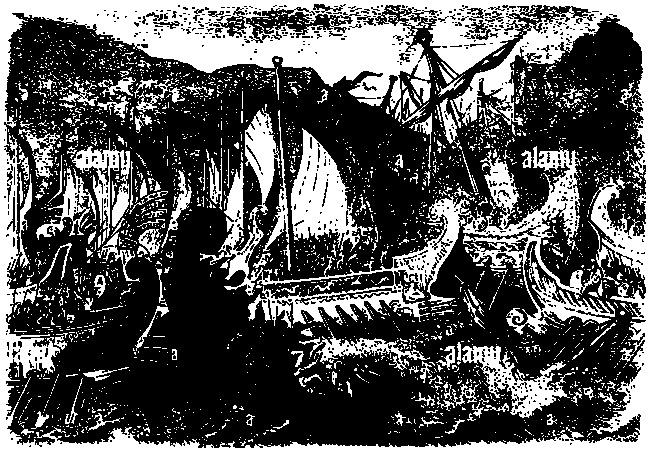
\includegraphics[width=\textwidth]{./images/combat11.pdf}
    % \caption{Inline Example Image}
\end{figure}

\subsection{Stabbing in The Abdomen}

\begin{description}[labelwidth=1.5em, leftmargin=*, itemsep=0.4em]
    \item[1 -] Minor abdominal scratch, slight discomfort. \textit{Recovery Time:} 1d4 hours. \textit{Scars:} Light scar.
    \item[2 -] Belly skin nicked, mild bleeding. \textit{Recovery Time:} 1d4 hours. \textit{Scars:} Small scar.
    \item[3 -] Navel area cut, minor pain and bleeding. \textit{Recovery Time:} 1d4 hours. \textit{Scars:} Tiny scar.
    \item[4 -] Side grazed, minor pain and discomfort. \textit{Recovery Time:} 1d4 hours. \textit{Scars:} Faint scar.
    \item[5 -] Lower abdomen cut, minor bleeding and irritation. \textit{Recovery Time:} 1d4 hours. \textit{Scars:} Light scar.
    \item[6 -] Hip scratched, slight bleeding. \textit{Recovery Time:} 1d4 hours. \textit{Scars:} Small scar.
    \item[7 -] Waistline cut, stinging pain and minor blood. \textit{Recovery Time:} 1d4 hours. \textit{Scars:} Tiny scar.
    \item[8 -] Upper abdomen wound, moderate pain and bleeding. \textit{Recovery Time:} 1d4 hours. \textit{Scars:} Faint scar.
    \item[9 -] Deep abdominal laceration, internal discomfort. \textit{Recovery Time:} 1d4 hours. \textit{Scars:} Light scar.
    \item[10 -] Flank cut, bleeding and mild pain. \textit{Recovery Time:} 1d4 hours. \textit{Scars:} Small scar.
    \item[11 -] Internal bleeding, urgent medical aid needed. \textit{Recovery Time:} 1d4 days. \textit{Scars:} Visible scar.
    \item[12 -] Peritonitis risk, prolonged medical attention. \textit{Recovery Time:} 1d4 days. \textit{Scars:} Disfiguring scar.
    \item[13 -] Critical hit, major organ punctured. \textit{Recovery Time:} Instant death. \textit{Scars:} N/A.
    \item[14 -] Critical hit, vital artery slashed. \textit{Recovery Time:} Instant death. \textit{Scars:} N/A.
    \item[15 -] Critical hit, massive internal bleeding. \textit{Recovery Time:} Instant death. \textit{Scars:} N/A.
    \item[16 -] Critical hit, organ rupture, instant death. \textit{Recovery Time:} Instant death. \textit{Scars:} N/A.
    \item[17 -] Critical hit, disembowelment, instant death. \textit{Recovery Time:} Instant death. \textit{Scars:} N/A.
    \item[18 -] Critical hit, abdominal explosion, instant death. \textit{Recovery Time:} Instant death. \textit{Scars:} N/A.
    \item[19 -] Critical hit, instant organ failure, instant death. \textit{Recovery Time:} Instant death. \textit{Scars:} N/A.
    \item[20 -] Critical hit, internal organs impaled, instant death. \textit{Recovery Time:} Instant death. \textit{Scars:} N/A.
\end{description}

\subsection{Stabbing in the Back}

\begin{description}[labelwidth=1.5em, leftmargin=*, itemsep=0.4em]
    \item[1 -] Superficial back scratch, minor discomfort. \textit{Recovery Time:} 1d4 hours. \textit{Scars:} Light scar.
    \item[2 -] Back skin nicked, slight bleeding. \textit{Recovery Time:} 1d4 hours. \textit{Scars:} Small scar.
    \item[3 -] Shoulder grazed, minor pain and irritation. \textit{Recovery Time:} 1d4 hours. \textit{Scars:} Tiny scar.
    \item[4 -] Lower back scratch, minor pain and discomfort. \textit{Recovery Time:} 1d4 hours. \textit{Scars:} Faint scar.
    \item[5 -] Spinal area cut, minor bleeding and irritation. \textit{Recovery Time:} 1d4 hours. \textit{Scars:} Light scar.
    \item[6 -] Upper back scratch, slight bleeding. \textit{Recovery Time:} 1d4 hours. \textit{Scars:} Small scar.
    \item[7 -] Mid-back cut, stinging pain and minor blood. \textit{Recovery Time:} 1d4 hours. \textit{Scars:} Tiny scar.
    \item[8 -] Deep back wound, moderate pain and bleeding. \textit{Recovery Time:} 1d4 hours. \textit{Scars:} Faint scar.
    \item[9 -] Punctured lung, labored breathing. \textit{Recovery Time:} 1d4 hours. \textit{Scars:} Light scar.
    \item[10 -] Kidney area cut, bleeding and mild pain. \textit{Recovery Time:} 1d4 hours. \textit{Scars:} Small scar.
    \item[11 -] Severed spine, instant paralysis. \textit{Recovery Time:} Instant death. \textit{Scars:} N/A.
    \item[12 -] Critical hit, major organ damage. \textit{Recovery Time:} Instant death. \textit{Scars:} N/A.
    \item[13 -] Critical hit, spinal cord severed. \textit{Recovery Time:} Instant death. \textit{Scars:} N/A.
    \item[14 -] Critical hit, internal bleeding. \textit{Recovery Time:} Instant death. \textit{Scars:} N/A.
    \item[15 -] Critical hit, vital artery punctured. \textit{Recovery Time:} Instant death. \textit{Scars:} N/A.
    \item[16 -] Critical hit, instant organ failure. \textit{Recovery Time:} Instant death. \textit{Scars:} N/A.
    \item[17 -] Critical hit, immediate paralysis. \textit{Recovery Time:} Instant death. \textit{Scars:} N/A.
    \item[18 -] Critical hit, internal damage, instant death. \textit{Recovery Time:} Instant death. \textit{Scars:} N/A.
    \item[19 -] Critical hit, catastrophic spine injury. \textit{Recovery Time:} Instant death. \textit{Scars:} N/A.
    \item[20 -] Critical hit, spine shattered, instant death. \textit{Recovery Time:} Instant death. \textit{Scars:} N/A.
\end{description}

\subsection{Stabbing in the Neck}

\begin{description}[labelwidth=1.5em, leftmargin=*, itemsep=0.4em]
    \item[1 -] Neck graze, minor pain and discomfort. \textit{Recovery Time:} 1d4 hours. \textit{Scars:} Light scar.
    \item[2 -] Shallow neck cut, slight bleeding. \textit{Recovery Time:} 1d4 hours. \textit{Scars:} Small scar.
    \item[3 -] Neck scratch, minor irritation. \textit{Recovery Time:} 1d4 hours. \textit{Scars:} Tiny scar.
    \item[4 -] Superficial neck wound, slight pain. \textit{Recovery Time:} 1d4 hours. \textit{Scars:} Faint scar.
    \item[5 -] Neck nicked, minor blood and discomfort. \textit{Recovery Time:} 1d4 hours. \textit{Scars:} Light scar.
    \item[6 -] Throat scratched, slight bleeding. \textit{Recovery Time:} 1d4 hours. \textit{Scars:} Small scar.
    \item[7 -] Neck cut, stinging pain and moderate bleeding. \textit{Recovery Time:} 1d4 hours. \textit{Scars:} Tiny scar.
    \item[8 -] Severe neck wound, bleeding and pain. \textit{Recovery Time:} 1d4 hours. \textit{Scars:} Faint scar.
    \item[9 -] Severed artery, immediate death. \textit{Recovery Time:} Instant death. \textit{Scars:} N/A.
    \item[10 -] Critical hit, major blood vessel hit. \textit{Recovery Time:} Instant death. \textit{Scars:} N/A.
    \item[11 -] Critical hit, spinal cord severed. \textit{Recovery Time:} Instant death. \textit{Scars:} N/A.
    \item[12 -] Critical hit, windpipe crushed. \textit{Recovery Time:} Instant death. \textit{Scars:} N/A.
    \item[13 -] Critical hit, jugular vein severed. \textit{Recovery Time:} Instant death. \textit{Scars:} N/A.
    \item[14 -] Critical hit, instant paralysis. \textit{Recovery Time:} Instant death. \textit{Scars:} N/A.
    \item[15 -] Critical hit, catastrophic bleeding. \textit{Recovery Time:} Instant death. \textit{Scars:} N/A.
    \item[16 -] Critical hit, severe pain and instant death. \textit{Recovery Time:} Instant death. \textit{Scars:} N/A.
    \item[17 -] Critical hit, airway blocked. \textit{Recovery Time:} Instant death. \textit{Scars:} N/A.
    \item[18 -] Critical hit, massive internal damage. \textit{Recovery Time:} Instant death. \textit{Scars:} N/A.
    \item[19 -] Critical hit, neck shattered. \textit{Recovery Time:} Instant death. \textit{Scars:} N/A.
    \item[20 -] Critical hit, decapitation. \textit{Recovery Time:} Instant death. \textit{Scars:} N/A.
\end{description}

\subsection{Stabbing in The Face}

\begin{description}[labelwidth=1.5em, leftmargin=*, itemsep=0.4em]
    \item[1 -] Facial graze, minor pain and discomfort. \textit{Recovery Time:} 1d4 hours. \textit{Scars:} Light scar.
    \item[2 -] Superficial cheek cut, slight bleeding. \textit{Recovery Time:} 1d4 hours. \textit{Scars:} Small scar.
    \item[3 -] Lip nicked, minor pain and bleeding. \textit{Recovery Time:} 1d4 hours. \textit{Scars:} Tiny scar.
    \item[4 -] Nostril scratched, minor irritation. \textit{Recovery Time:} 1d4 hours. \textit{Scars:} Faint scar.
    \item[5 -] Eyebrow cut, minor blood and discomfort. \textit{Recovery Time:} 1d4 hours. \textit{Scars:} Light scar.
    \item[6 -] Chin scratched, slight bleeding. \textit{Recovery Time:} 1d4 hours. \textit{Scars:} Small scar.
    \item[7 -] Jaw cut, stinging pain and minor bleeding. \textit{Recovery Time:} 1d4 hours. \textit{Scars:} Tiny scar.
    \item[8 -] Forehead gash, bleeding and moderate pain. \textit{Recovery Time:} 1d4 hours. \textit{Scars:} Faint scar.
    \item[9 -] Eye injured, risk of blindness. \textit{Recovery Time:} 1d4 days. \textit{Scars:} Disfiguring scar.
    \item[10 -] Deep facial wound, potential scarring. \textit{Recovery Time:} 1d4 days. \textit{Scars:} Visible scar.
    \item[11 -] Skull fracture, severe headache. \textit{Recovery Time:} 1d4 weeks. \textit{Scars:} Permanent damage.
    \item[12 -] Head gash, risk of infection. \textit{Recovery Time:} 1d4 weeks. \textit{Scars:} Deep scar.
    \item[13 -] Critical hit, brain damage. \textit{Recovery Time:} Instant death. \textit{Scars:} N/A.
    \item[14 -] Critical hit, facial disfigurement. \textit{Recovery Time:} Instant death. \textit{Scars:} N/A.
    \item[15 -] Critical hit, severed nerve. \textit{Recovery Time:} Instant death. \textit{Scars:} N/A.
    \item[16 -] Critical hit, eye punctured. \textit{Recovery Time:} Instant death. \textit{Scars:} N/A.
    \item[17 -] Critical hit, shattered jaw. \textit{Recovery Time:} Instant death. \textit{Scars:} N/A.
    \item[18 -] Critical hit, facial collapse. \textit{Recovery Time:} Instant death. \textit{Scars:} N/A.
    \item[19 -] Critical hit, extreme blood loss. \textit{Recovery Time:} Instant death. \textit{Scars:} N/A.
    \item[20 -] Critical hit, facial mutilation. \textit{Recovery Time:} Instant death. \textit{Scars:} N/A.
\end{description}

\begin{figure}[h]
    \centering
    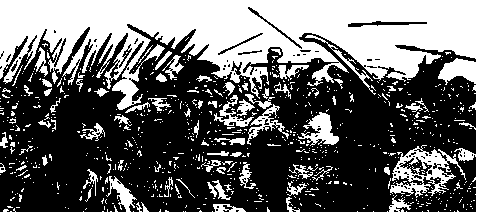
\includegraphics[width=\textwidth]{./images/combat12.pdf}
    % \caption{Inline Example Image}
\end{figure}

\subsection{Impact in the Head}

\begin{description}[labelwidth=1.5em, leftmargin=*, itemsep=0.4em]
    \item[1 -] Light head bump, minor discomfort \textit{Recovery Time:} 1d4 hours. \textit{Scars:} N/A.
    \item[2 -] Forehead knock, slight headache \textit{Recovery Time:} 1d4 hours. \textit{Scars:} N/A.
    \item[3 -] Ear hit, temporary ringing and pain \textit{Recovery Time:} 1d4 hours. \textit{Scars:} N/A.
    \item[4 -] Nose impact, minor bleeding and discomfort \textit{Recovery Time:} 1d4 hours. \textit{Scars:} N/A.
    \item[5 -] Crown hit, momentary dizziness \textit{Recovery Time:} 1d4 hours. \textit{Scars:} N/A.
    \item[6 -] Cheek strike, slight swelling \textit{Recovery Time:} 1d4 hours. \textit{Scars:} N/A.
    \item[7 -] Chin impact, stinging pain \textit{Recovery Time:} 1d4 hours. \textit{Scars:} N/A.
    \item[8 -] Temple bump, moderate headache \textit{Recovery Time:} 1d4 hours. \textit{Scars:} N/A.
    \item[9 -] Face slam, disoriented and headache \textit{Recovery Time:} 1d4 hours. \textit{Scars:} N/A.
    \item[10 -] Eye socket hit, risk of vision issues \textit{Recovery Time:} 1d4 days. \textit{Scars:} N/A.
    \item[11 -] Skull jolt, potential for migraines \textit{Recovery Time:} 1d4 days. \textit{Scars:} N/A.
    \item[12 -] Facial fracture, severe pain \textit{Recovery Time:} 1d4 weeks. \textit{Scars:} N/A.
    \item[13 -] Head impact, risk of concussion \textit{Recovery Time:} 1d4 weeks. \textit{Scars:} N/A.
    \item[14 -] Severe brain trauma, unconsciousness \textit{Recovery Time:} 1d4 weeks. \textit{Scars:} N/A.
    \item[15 -] Critical hit, cranial collapse \textit{Recovery Time:} Instant death. \textit{Scars:} N/A.
    \item[16 -] Critical hit, brain rupture \textit{Recovery Time:} Instant death. \textit{Scars:} N/A.
    \item[17 -] Critical hit, instant brain death \textit{Recovery Time:} Instant death. \textit{Scars:} N/A.
    \item[18 -] Critical hit, skull shattered \textit{Recovery Time:} Instant death. \textit{Scars:} N/A.
    \item[19 -] Critical hit, massive internal bleeding \textit{Recovery Time:} Instant death. \textit{Scars:} N/A.
    \item[20 -] Critical hit, head explosion \textit{Recovery Time:} Instant death. \textit{Scars:} N/A.
\end{description}

\subsection{Impact in the Torso}

\begin{description}[labelwidth=1.5em, leftmargin=*, itemsep=0.4em]
    \item[1 -] Bruised ribs, mild discomfort \textit{Recovery Time:} 1d4 hours. \textit{Scars:} N/A.
    \item[2 -] Solar plexus hit, shortness of breath \textit{Recovery Time:} 1d4 hours. \textit{Scars:} N/A.
    \item[3 -] Abdominal punch, temporary nausea \textit{Recovery Time:} 1d4 hours. \textit{Scars:} N/A.
    \item[4 -] Lower rib impact, minor pain \textit{Recovery Time:} 1d4 hours. \textit{Scars:} N/A.
    \item[5 -] Sides struck, momentary weakness \textit{Recovery Time:} 1d4 hours. \textit{Scars:} N/A.
    \item[6 -] Upper abdomen blow, slight swelling \textit{Recovery Time:} 1d4 hours. \textit{Scars:} N/A.
    \item[7 -] Diaphragm hit, difficulty breathing \textit{Recovery Time:} 1d4 hours. \textit{Scars:} N/A.
    \item[8 -] Sternum impact, moderate discomfort \textit{Recovery Time:} 1d4 hours. \textit{Scars:} N/A.
    \item[9 -] Rib cage shock, disorientation \textit{Recovery Time:} 1d4 hours. \textit{Scars:} N/A.
    \item[10 -] Organ bruise, potential complications \textit{Recovery Time:} 1d4 days. \textit{Scars:} N/A.
    \item[11 -] Internal bleeding, risk of infection \textit{Recovery Time:} 1d4 days. \textit{Scars:} N/A.
    \item[12 -] Rib fracture, severe pain \textit{Recovery Time:} 1d4 weeks. \textit{Scars:} N/A.
    \item[13 -] Spleen or liver damage, risk of shock \textit{Recovery Time:} 1d4 weeks. \textit{Scars:} N/A.
    \item[14 -] Critical hit, vital organ rupture \textit{Recovery Time:} Instant death. \textit{Scars:} N/A.
    \item[15 -] Critical hit, cardiac arrest \textit{Recovery Time:} Instant death. \textit{Scars:} N/A.
    \item[16 -] Critical hit, internal organs obliterated \textit{Recovery Time:} Instant death. \textit{Scars:} N/A.
    \item[17 -] Critical hit, massive hemorrhage \textit{Recovery Time:} Instant death. \textit{Scars:} N/A.
    \item[18 -] Critical hit, torso shattered \textit{Recovery Time:} Instant death. \textit{Scars:} N/A.
    \item[19 -] Critical hit, torso explosion \textit{Recovery Time:} Instant death. \textit{Scars:} N/A.
    \item[20 -] Critical hit, instant torso disintegration \textit{Recovery Time:} Instant death. \textit{Scars:} N/A.
\end{description}

\subsection{Impact in the Arms}

\begin{description}[labelwidth=1.5em, leftmargin=*, itemsep=0.4em]
    \item[1 -] Minor bruising, mild discomfort \textit{Recovery Time:} 1d4 hours. \textit{Scars:} N/A.
    \item[2 -] Elbow knock, slight soreness \textit{Recovery Time:} 1d4 hours. \textit{Scars:} N/A.
    \item[3 -] Forearm hit, temporary weakness \textit{Recovery Time:} 1d4 hours. \textit{Scars:} N/A.
    \item[4 -] Wrist impact, minor pain and stiffness \textit{Recovery Time:} 1d4 hours. \textit{Scars:} N/A.
    \item[5 -] Hand struck, momentary numbness \textit{Recovery Time:} 1d4 hours. \textit{Scars:} N/A.
    \item[6 -] Fingers jammed, slight swelling \textit{Recovery Time:} 1d4 hours. \textit{Scars:} N/A.
    \item[7 -] Shoulder impact, stinging pain \textit{Recovery Time:} 1d4 hours. \textit{Scars:} N/A.
    \item[8 -] Upper arm blow, moderate discomfort \textit{Recovery Time:} 1d4 hours. \textit{Scars:} N/A.
    \item[9 -] Dislocated joint, risk of complications \textit{Recovery Time:} 1d4 days. \textit{Scars:} N/A.
    \item[10 -] Fractured bone, potential for deformity \textit{Recovery Time:} 1d4 days. \textit{Scars:} N/A.
    \item[11 -] Severely dislocated joint, loss of function \textit{Recovery Time:} 1d4 weeks. \textit{Scars:} N/A.
    \item[12 -] Arm bone shattered, severe pain \textit{Recovery Time:} 1d4 weeks. \textit{Scars:} N/A.
    \item[13 -] Critical hit, arm amputation \textit{Recovery Time:} Instant death. \textit{Scars:} N/A.
    \item[14 -] Critical hit, shattered arm \textit{Recovery Time:} Instant death. \textit{Scars:} N/A.
    \item[15 -] Critical hit, arm obliteration \textit{Recovery Time:} Instant death. \textit{Scars:} N/A.
    \item[16 -] Critical hit, arm torn off \textit{Recovery Time:} Instant death. \textit{Scars:} N/A.
    \item[17 -] Critical hit, massive arm hemorrhage \textit{Recovery Time:} Instant death. \textit{Scars:} N/A.
    \item[18 -] Critical hit, arm explosion \textit{Recovery Time:} Instant death. \textit{Scars:} N/A.
    \item[19 -] Critical hit, instant arm disintegration \textit{Recovery Time:} Instant death. \textit{Scars:} N/A.
    \item[20 -] Critical hit, arm vaporization \textit{Recovery Time:} Instant death. \textit{Scars:} N/A.
\end{description}

\begin{figure}[h]
    \centering
    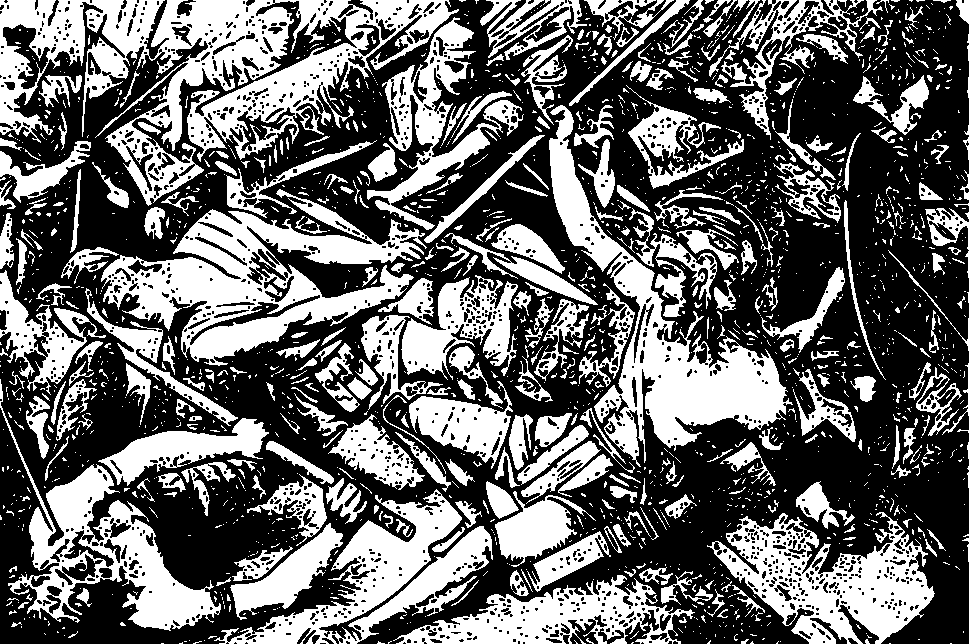
\includegraphics[width=\textwidth]{./images/combat13.pdf}
    % \caption{Inline Example Image}
\end{figure}

\subsection{Impact in the Legs}

\begin{description}[labelwidth=1.5em, leftmargin=*, itemsep=0.4em]
    \item[1 -] Minor shin bump, slight discomfort \textit{Recovery Time:} 1d4 hours. \textit{Scars:} N/A.
    \item[2 -] Knee hit, temporary limping \textit{Recovery Time:} 1d4 hours. \textit{Scars:} N/A.
    \item[3 -] Thigh impact, momentary weakness \textit{Recovery Time:} 1d4 hours. \textit{Scars:} N/A.
    \item[4 -] Calf struck, minor pain and stiffness \textit{Recovery Time:} 1d4 hours. \textit{Scars:} N/A.
    \item[5 -] Ankle twisted, brief numbness \textit{Recovery Time:} 1d4 hours. \textit{Scars:} N/A.
    \item[6 -] Foot stepped on, slight swelling \textit{Recovery Time:} 1d4 hours. \textit{Scars:} N/A.
    \item[7 -] Groin impact, stinging pain \textit{Recovery Time:} 1d4 hours. \textit{Scars:} N/A.
    \item[8 -] Upper leg blow, moderate discomfort \textit{Recovery Time:} 1d4 hours. \textit{Scars:} N/A.
    \item[9 -] Dislocated joint, risk of complications \textit{Recovery Time:} 1d4 days. \textit{Scars:} N/A.
    \item[10 -] Fractured bone, potential for deformity \textit{Recovery Time:} 1d4 days. \textit{Scars:} N/A.
    \item[11 -] Severely dislocated joint, loss of function \textit{Recovery Time:} 1d4 weeks. \textit{Scars:} N/A.
    \item[12 -] Leg bone shattered, severe pain \textit{Recovery Time:} 1d4 weeks. \textit{Scars:} N/A.
    \item[13 -] Critical hit, leg amputation \textit{Recovery Time:} Instant death. \textit{Scars:} N/A.
    \item[14 -] Critical hit, shattered leg \textit{Recovery Time:} Instant death. \textit{Scars:} N/A.
    \item[15 -] Critical hit, leg obliteration \textit{Recovery Time:} Instant death. \textit{Scars:} N/A.
    \item[16 -] Critical hit, leg torn off \textit{Recovery Time:} Instant death. \textit{Scars:} N/A.
    \item[17 -] Critical hit, massive leg hemorrhage \textit{Recovery Time:} Instant death. \textit{Scars:} N/A.
    \item[18 -] Critical hit, leg explosion \textit{Recovery Time:} Instant death. \textit{Scars:} N/A.
    \item[19 -] Critical hit, instant leg disintegration \textit{Recovery Time:} Instant death. \textit{Scars:} N/A.
    \item[20 -] Critical hit, leg vaporization \textit{Recovery Time:} Instant death. \textit{Scars:} N/A.
\end{description}

\subsection{Impact on Abdomen}

\begin{description}[labelwidth=1.5em, leftmargin=*, itemsep=0.4em]
    \item[1 -] Minor abdomen bump, slight discomfort \textit{Recovery Time:} 1d4 hours. \textit{Scars:} N/A.
    \item[2 -] Belly hit, brief nausea \textit{Recovery Time:} 1d4 hours. \textit{Scars:} N/A.
    \item[3 -] Midriff impact, momentary weakness \textit{Recovery Time:} 1d4 hours. \textit{Scars:} N/A.
    \item[4 -] Lower abdomen struck, minor pain \textit{Recovery Time:} 1d4 hours. \textit{Scars:} N/A.
    \item[5 -] Side blow, temporary numbness \textit{Recovery Time:} 1d4 hours. \textit{Scars:} N/A.
    \item[6 -] Groin strike, slight swelling \textit{Recovery Time:} 1d4 hours. \textit{Scars:} N/A.
    \item[7 -] Kidney impact, stinging pain \textit{Recovery Time:} 1d4 hours. \textit{Scars:} N/A.
    \item[8 -] Abdominal blow, moderate discomfort \textit{Recovery Time:} 1d4 hours. \textit{Scars:} N/A.
    \item[9 -] Organ damage, risk of complications \textit{Recovery Time:} 1d4 days. \textit{Scars:} N/A.
    \item[10 -] Internal bleeding, potential for infection \textit{Recovery Time:} 1d4 days. \textit{Scars:} N/A.
    \item[11 -] Ruptured organ, severe pain \textit{Recovery Time:} 1d4 weeks. \textit{Scars:} N/A.
    \item[12 -] Abdominal cavity breached, severe internal injuries \textit{Recovery Time:} 1d4 weeks. \textit{Scars:} N/A.
    \item[13 -] Critical hit, vital organ rupture \textit{Recovery Time:} Instant death. \textit{Scars:} N/A.
    \item[14 -] Critical hit, abdominal obliteration \textit{Recovery Time:} Instant death. \textit{Scars:} N/A.
    \item[15 -] Critical hit, massive internal hemorrhage \textit{Recovery Time:} Instant death. \textit{Scars:} N/A.
    \item[16 -] Critical hit, abdominal explosion \textit{Recovery Time:} Instant death. \textit{Scars:} N/A.
    \item[17 -] Critical hit, instant abdominal disintegration \textit{Recovery Time:} Instant death. \textit{Scars:} N/A.
    \item[18 -] Critical hit, abdominal vaporization \textit{Recovery Time:} Instant death. \textit{Scars:} N/A.
    \item[19 -] Critical hit, instant abdominal implosion \textit{Recovery Time:} Instant death. \textit{Scars:} N/A.
    \item[20 -] Critical hit, abdominal annihilation \textit{Recovery Time:} Instant death. \textit{Scars:} N/A.
\end{description}

\begin{figure}[h]
    \centering
    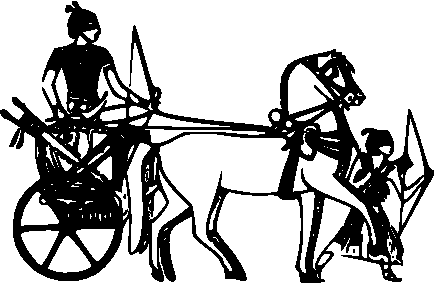
\includegraphics[width=\textwidth]{./images/combat14.pdf}
    % \caption{Inline Example Image}
\end{figure}

\subsection{Impact on Neck}

\begin{description}[labelwidth=1.5em, leftmargin=*, itemsep=0.4em]
    \item[1 -] Neck graze, minor pain and discomfort \textit{Recovery Time:} 1d4 hours. \textit{Scars:} N/A.
    \item[2 -] Throat hit, momentary choking sensation \textit{Recovery Time:} 1d4 hours. \textit{Scars:} N/A.
    \item[3 -] Neck blow, temporary loss of breath \textit{Recovery Time:} 1d4 hours. \textit{Scars:} N/A.
    \item[4 -] Collarbone impact, slight discomfort \textit{Recovery Time:} 1d4 hours. \textit{Scars:} N/A.
    \item[5 -] Jaw struck, temporary jaw numbness \textit{Recovery Time:} 1d4 hours. \textit{Scars:} N/A.
    \item[6 -] Neck muscle hit, slight pain \textit{Recovery Time:} 1d4 hours. \textit{Scars:} N/A.
    \item[7 -] Adam's apple impact, painful swallowing \textit{Recovery Time:} 1d4 hours. \textit{Scars:} N/A.
    \item[8 -] Neck shock, moderate discomfort \textit{Recovery Time:} 1d4 hours. \textit{Scars:} N/A.
    \item[9 -] Choking risk, risk of complications \textit{Recovery Time:} 1d4 days. \textit{Scars:} N/A.
    \item[10 -] Collarbone fracture, potential for deformity \textit{Recovery Time:} 1d4 days. \textit{Scars:} N/A.
    \item[11 -] Severe neck injury, difficulty in breathing \textit{Recovery Time:} 1d4 weeks. \textit{Scars:} N/A.
    \item[12 -] Neck fracture, severe pain \textit{Recovery Time:} 1d4 weeks. \textit{Scars:} N/A.
    \item[13 -] Critical hit, trachea rupture \textit{Recovery Time:} Instant death. \textit{Scars:} N/A.
    \item[14 -] Critical hit, neck obliteration \textit{Recovery Time:} Instant death. \textit{Scars:} N/A.
    \item[15 -] Critical hit, severe internal bleeding \textit{Recovery Time:} Instant death. \textit{Scars:} N/A.
    \item[16 -] Critical hit, neck explosion \textit{Recovery Time:} Instant death. \textit{Scars:} N/A.
    \item[17 -] Critical hit, instant neck disintegration \textit{Recovery Time:} Instant death. \textit{Scars:} N/A.
    \item[18 -] Critical hit, neck vaporization \textit{Recovery Time:} Instant death. \textit{Scars:} N/A.
    \item[19 -] Critical hit, instant neck implosion \textit{Recovery Time:} Instant death. \textit{Scars:} N/A.
    \item[20 -] Critical hit, neck annihilation \textit{Recovery Time:} Instant death. \textit{Scars:} N/A.
\end{description}

\begin{figure}[h]
    \centering
    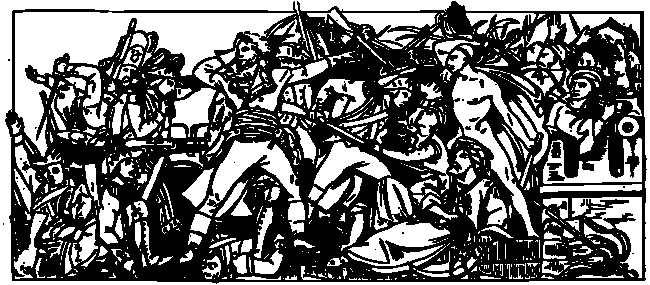
\includegraphics[width=\textwidth]{./images/combat17.pdf}
    % \caption{Inline Example Image}
\end{figure}

\subsection{Impact on Face}

\begin{description}[labelwidth=1.5em, leftmargin=*, itemsep=0.4em]
    \item[1 -] Facial graze, minor pain and discomfort \textit{Recovery Time:} 1d4 hours. \textit{Scars:} Light scar.
    \item[2 -] Superficial cheek cut, slight bleeding \textit{Recovery Time:} 1d4 hours. \textit{Scars:} Small scar.
    \item[3 -] Lip nicked, minor pain and bleeding \textit{Recovery Time:} 1d4 hours. \textit{Scars:} Tiny scar.
    \item[4 -] Nostril scratched, minor irritation \textit{Recovery Time:} 1d4 hours. \textit{Scars:} Faint scar.
    \item[5 -] Eyebrow cut, minor blood and discomfort \textit{Recovery Time:} 1d4 hours. \textit{Scars:} Light scar.
    \item[6 -] Chin scratched, slight bleeding \textit{Recovery Time:} 1d4 hours. \textit{Scars:} Small scar.
    \item[7 -] Jaw cut, stinging pain and minor bleeding \textit{Recovery Time:} 1d4 hours. \textit{Scars:} Tiny scar.
    \item[8 -] Forehead gash, bleeding and moderate pain \textit{Recovery Time:} 1d4 hours. \textit{Scars:} Faint scar.
    \item[9 -] Eye injured, risk of blindness \textit{Recovery Time:} 1d4 days. \textit{Scars:} Disfiguring scar.
    \item[10 -] Deep facial wound, potential scarring \textit{Recovery Time:} 1d4 days. \textit{Scars:} Visible scar.
    \item[11 -] Skull fracture, severe headache \textit{Recovery Time:} 1d4 weeks. \textit{Scars:} Permanent damage.
    \item[12 -] Head gash, risk of infection \textit{Recovery Time:} 1d4 weeks. \textit{Scars:} Deep scar.
    \item[13 -] Critical hit, brain damage \textit{Recovery Time:} Instant death. \textit{Scars:} N/A.
    \item[14 -] Critical hit, facial disfigurement \textit{Recovery Time:} Instant death. \textit{Scars:} N/A.
    \item[15 -] Critical hit, severed nerve \textit{Recovery Time:} Instant death. \textit{Scars:} N/A.
    \item[16 -] Critical hit, eye punctured \textit{Recovery Time:} Instant death. \textit{Scars:} N/A.
    \item[17 -] Critical hit, shattered jaw \textit{Recovery Time:} Instant death. \textit{Scars:} N/A.
    \item[18 -] Critical hit, facial collapse \textit{Recovery Time:} Instant death. \textit{Scars:} N/A.
    \item[19 -] Critical hit, extreme blood loss \textit{Recovery Time:} Instant death. \textit{Scars:} N/A.
    \item[20 -] Critical hit, facial mutilation \textit{Recovery Time:} Instant death. \textit{Scars:} N/A.
\end{description}

\subsection{Impact on the Back}

\begin{description}[labelwidth=1.5em, leftmargin=*, itemsep=0.4em]
    \item[1 -] Surface bruise, mild discomfort \textit{Recovery Time:} 1d4 hours. \textit{Scars:} N/A.
    \item[2 -] Lower back hit, temporary stiffness \textit{Recovery Time:} 1d4 hours. \textit{Scars:} N/A.
    \item[3 -] Mid-back blow, momentary pain \textit{Recovery Time:} 1d4 hours. \textit{Scars:} N/A.
    \item[4 -] Upper back impact, mild soreness \textit{Recovery Time:} 1d4 hours. \textit{Scars:} N/A.
    \item[5 -] Side strike, brief numbness \textit{Recovery Time:} 1d4 hours. \textit{Scars:} N/A.
    \item[6 -] Spine hit, slight discomfort \textit{Recovery Time:} 1d4 hours. \textit{Scars:} N/A.
    \item[7 -] Kidney shock, sharp pain \textit{Recovery Time:} 1d4 hours. \textit{Scars:} N/A.
    \item[8 -] Back thump, moderate discomfort \textit{Recovery Time:} 1d4 hours. \textit{Scars:} N/A.
    \item[9 -] Spinal strain, risk of complications \textit{Recovery Time:} 1d4 days. \textit{Scars:} N/A.
    \item[10 -] Vertebral fracture, potential nerve damage \textit{Recovery Time:} 1d4 days. \textit{Scars:} N/A.
    \item[11 -] Severe back injury, difficulty in movement \textit{Recovery Time:} 1d4 weeks. \textit{Scars:} N/A.
    \item[12 -] Disc herniation, severe pain \textit{Recovery Time:} 1d4 weeks. \textit{Scars:} N/A.
    \item[13 -] Critical hit, spinal cord damage \textit{Recovery Time:} Instant death. \textit{Scars:} N/A.
    \item[14 -] Critical hit, back obliteration \textit{Recovery Time:} Instant death. \textit{Scars:} N/A.
    \item[15 -] Critical hit, catastrophic internal damage \textit{Recovery Time:} Instant death. \textit{Scars:} N/A.
    \item[16 -] Critical hit, vertebral explosion \textit{Recovery Time:} Instant death. \textit{Scars:} N/A.
    \item[17 -] Critical hit, instant back disintegration \textit{Recovery Time:} Instant death. \textit{Scars:} N/A.
    \item[18 -] Critical hit, back vaporization \textit{Recovery Time:} Instant death. \textit{Scars:} N/A.
    \item[19 -] Critical hit, instant back implosion \textit{Recovery Time:} Instant death. \textit{Scars:} N/A.
    \item[20 -] Critical hit, back annihilation \textit{Recovery Time:} Instant death. \textit{Scars:} N/A.
\end{description}

\begin{figure}[h]
    \centering
    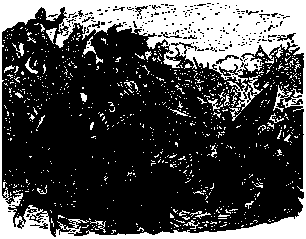
\includegraphics[width=\textwidth]{./images/combat16.pdf}
    % \caption{Inline Example Image}
\end{figure}

\subsection{Fire Injuries}

Fire is a potent force on the battlefield, capable of causing devastating injuries and leaving lasting scars. Whether from a raging inferno or a targeted spell, fire damage can result in a variety of effects, including:

\begin{itemize}
    \item \textbf{Burns}: Characters may suffer from first-degree burns, causing pain and discomfort but relatively minor damage. More severe burns, such as second or third-degree burns, can lead to blistering, tissue damage, and long-term complications.
    \item \textbf{Smoke Inhalation}: In addition to direct flame exposure, individuals caught in fires may inhale smoke, leading to respiratory issues, coughing, and reduced lung function.
    \item \textbf{Environmental Hazards}: Fires can spread rapidly, creating hazardous conditions such as collapsing structures, intense heat, and limited visibility.
\end{itemize}

\subsection{Acid}

Acid poses a different set of challenges, corroding flesh, armor, and equipment with its caustic properties. When subjected to acid attacks, characters must contend with the following hazards:

\textbf{Types of Acid Damage}

\begin{itemize}
    \item \textbf{Corrosive Burns}: Acid eats away at organic and inorganic materials alike, causing painful burns and potentially permanent damage to skin, clothing, and gear.
    \item \textbf{Armor Degradation}: Protective armor may suffer from corrosion, compromising its integrity and reducing its effectiveness in defending against future attacks.
    \item \textbf{Environmental Contamination}: Pools of acid or acidic fumes can create hazardous environments, posing risks to both health and equipment.
\end{itemize}

\subsection{Poison}

Poison introduces a stealthy and insidious threat to adventurers, lurking in traps, tainted food, or the fangs of venomous creatures. Unlike conventional damage, poison affects its victims over time, gradually weakening their bodies and impairing their abilities.

\textbf{Types of Poison}

\begin{itemize}
    \item \textbf{Contact Poison}: Applied to weapons or surfaces, contact poisons require physical contact to take effect, such as through a poisoned blade or a booby-trapped object.
    \item \textbf{Ingested Poison}: Consumed through food or drink, ingested poisons target the digestive system, leading to nausea, vomiting, and systemic damage.
    \item \textbf{Inhaled Poison}: Released as gas or vapor, inhaled poisons affect the respiratory system, causing coughing, difficulty breathing, and potentially lethal asphyxiation.
    \item \textbf{Injected Poison}: Delivered via puncture wounds, injected poisons are typically associated with venomous creatures, such as snakes or spiders, and can induce paralysis, organ failure, or death.
\end{itemize}

\subsection{Instant Death and Recovery}

In some instances, the outcome of an attack can lead to instant death if the damage dealt is significant enough. Eidos doesn't shy away from the gravity of battle.
For non-fatal injuries, a period of recovery follows. Players who emerge victorious or disengage from the conflict can recuperate over time. The aftermath of combat may leave scars or lingering effects, adding depth to your character's journey.

The aftermath of combat extends beyond the battlefield. Players who survive are left to recover from their wounds, with lasting scars as tokens of their trials. The scars serve as reminders of battles fought, adding layers of realism and immersion to the world of Eidos.
As you continue your exploration of this system, embrace the intricate interplay of choice, strategy, and chance that defines Eidos' unique combat and conflict resolution mechanics.



